\begin{figure}[t]
\uwsinglespace
\begin{center}
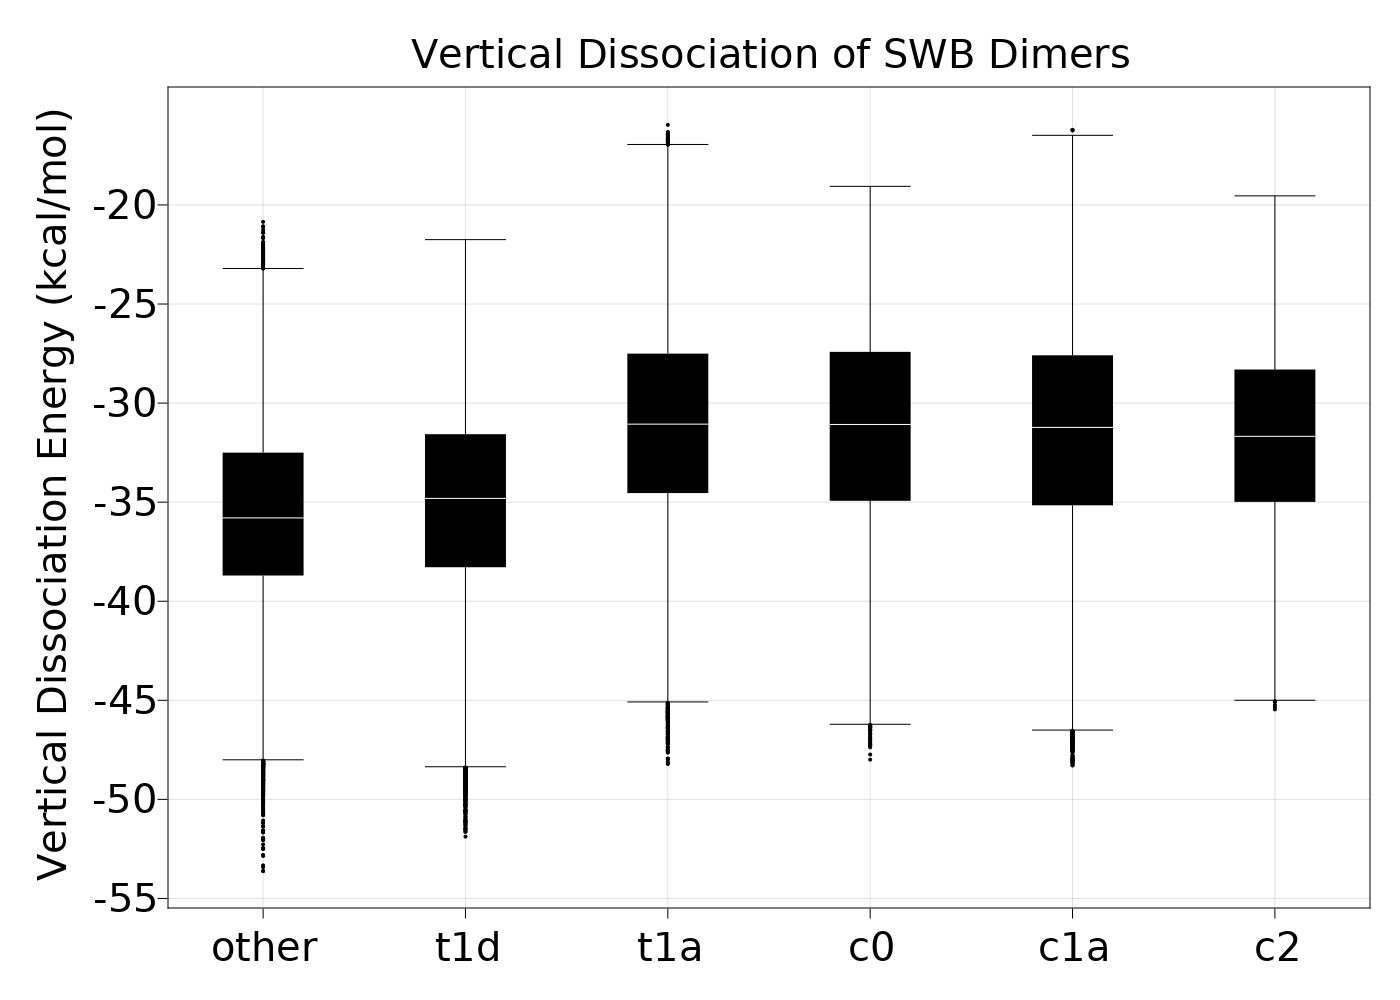
\includegraphics[width=.9\textwidth]{Figures/Chapter_6/w20_clathrate_vertical_dissociation_dimers.png}
\end{center}
\begin{spacing}{1.0}
\caption[Vertical dissociation energy (see text for details) of all dimers from all 30,026 optimized \ce{(H2O)_{20}} clathrate cages. Note that t1d dimers are about 3 kcal/mol more stable than all other types of dimers, on average, while all other SWEB dimers are similarly stable. The non-SWEB dimers present in collapsed cages are of slightly more stable than t1d dimers on average.]{Vertical dissociation energy (see text for details) of all dimers from all 30,026 optimized \ce{(H2O)_{20}} clathrate cages. Note that t1d dimers are about 3 kcal/mol more stable than all other types of dimers, on average, while all other SWEB dimers are similarly stable. The non-SWEB dimers present in collapsed cages are of slightly more stable than t1d dimers on average.}\label{fig:MBE_III_F4}
\end{spacing}
\end{figure}